\chapter[Attacco di de-anonimizzazione]{Validazione sperimentale: Attacco di de-anonimizzazione}

In questo capitolo si procede ad illustrare un caso di utilizzo di GoDP con l'obiettivo di dimostrare l'efficacia della privacy differenziale contro attacchi di de-anonimizzazione. L'esperimento simula uno scenario realistico in cui un attaccante tenta di dedurre informazioni sensibili su un individuo specifico a partire da aggregazioni su un dataset, confrontando i risultati ottenuti con e senza l'applicazione di meccanismi differenzialmente privati.

\section{Threat model}

L'esperimento si basa sul modello di privacy differenziale \textit{centralizzato}, nel quale un \textit{curatore} fidato ha accesso al database in chiaro e agisce come intermediario tra la sorgente dei dati e gli analisti che desiderano effettuare query aggregate sul dataset. Il curatore riceve le richieste di aggregazione, applica un meccanismo DP opportunamente calibrato e restituisce il risultato protetto dalle garanzie della privacy differenziale.

Nel contesto di questo modello di applicazione della DP, si identificano quattro attori principali:
\begin{itemize}
    \item \textbf{dataset originale}, contenente i dati sensibili dei dipendenti di un'azienda in chiaro e reso accessibile esclusivamente al curatore fidato;
    \item \textbf{curatore};
    \item \textbf{analista} e
    \item \textbf{attaccante}.
\end{itemize}

L'\textit{analista} è un soggetto che utilizza il sistema di interrogazione del database allo scopo di analizzare i dati contenuti, mentre l'\textit{attaccante} è un analista malintenzionato che ha a disposizione informazioni ausiliarie sulla vittima raccolte da fonti esterne, come ad esempio piattaforme di social networking, o ottenute tramite tecniche di social engineering. Il \textit{curatore} è l'entità fidata che implementa e applica il meccanismo DP: riceve le query, aggiunge rumore calibrato e restituisce risultati differenzialmente privati.

Il threat model si basa su alcune assunzioni fondamentali:
\begin{itemize}
    \item il curatore è fidato e non collude con l'attaccante
    \item l'attaccante non può manomettere o corrompere il sistema che implementa il meccanismo DP
    \item gli analisti possono osservare esclusivamente i risultati differenzialmente privati; non hanno accesso diretto ai dati grezzi del dataset
    \item l'attaccante può avere accesso a informazioni ausiliarie sulla vittima ottenute da fonti esterne
    \item l'attaccante conosce la struttura del dataset, ovvero gli attributi che il dataset contiene; queste informazioni sono necessariamente pubbliche per permettere un accesso efficace da parte degli analisti
\end{itemize}

%cosa può conoscere l'attaccante (modello DP resistente a):
%conoscenza schema dataset
%conoscenza meccanismo M
%conoscenza budget di privacy

\begin{figure}[H]
    \centering
    
\includegraphics[scale=0.6]{plots/centralized_dp_model.pdf}
    \caption{Modello DP centralizzata}
\end{figure}

\section{Difference attack}

Il \textit{difference attack} è una tecnica di de-anonimizzazione che permette a un attaccante di dedurre informazioni sensibili su un singolo individuo combinando i risultati di più query aggregate. L'attacco sfrutta il fatto che le aggregazioni esatte permettono di isolare il contributo di un individuo specifico attraverso sottrazioni successive. \cite{TCS-042}

Sia $D$ un dataset e $f$ una funzione di aggregazione (e.g. somma, conteggio, media...); l'attaccante identifica due sottoinsiemi:
\begin{itemize}
    \item $D_{\text{include}}$, che include la vittima target e
    \item $D_{\text{exclude}}$, lo stesso sottoinsieme senza la vittima
\end{itemize}

\noindent
Il valore associato alla vittima può essere calcolato come:
\begin{equation}
    \text{record}_{\text{vittima}} = f(D_{\text{include}} - D_{\text{exclude}})
    \label{eq:differencing_attack}
\end{equation}

Allo scopo di illustrare l'efficacia del difference attack, si considera un sistema che sfrutta una tecnica di protezione basata su una \textit{soglia minima di aggregazione}, questo metodo impone che il sistema rifiuti di restituire qualsiasi risultato quando il numero di record che soddisfa i criteri della query è inferiore a una costante $k$. Questo meccanismo, noto come \textit{suppression threshold}, è ampiamente utilizzato in sistemi statistici reali come protezione contro la re-identificazione \cite{kThreshold}.

In presenza di tale meccanismo, una query che filtra per tutti gli attributi noti della vittima verrebbe rifiutata dal sistema, in quanto restituirebbe un singolo record ($1 < k$). L'attaccante è quindi costretto a ricorrere al difference attack: interrogando il sistema con query che coinvolgono gruppi sufficientemente numerosi da superare la soglia $k$, e calcolando differenze tra i risultati, può aggirare la protezione e isolare il contributo della vittima. Questo scenario dimostra come la soglia minima di aggregazione, pur offrendo un certo livello di protezione, sia vulnerabile ad attacchi che sfruttano conoscenze ausiliarie sui membri del dataset. Per gli scopi di questo esperimento si utilizzerà una costante $k = 5$ ($~ 1\%$ dataset).

Tenendo conto delle informazioni ausiliarie a disposizione dell'attaccante, egli procede a interrogare il sistema tramite una serie di query specifiche che gli permettono di restringere progressivamente l'insieme dei record considerati fino a isolare il record contenente le informazioni della vittima.

L'attaccante inizia interrogando il sistema per ottenere la somma totale degli stipendi del reparto della vittima.
\begin{equation}
    S_1 = \text{SUM(Salary) WHERE Department = 'Engineering'}
\end{equation}
Successivamente, esclude i dipendenti che hanno la stessa età della vittima con una seconda query.
\begin{equation}
    S_2 = \text{SUM(Salary) WHERE Department = 'Engineering'} \ \land \ \text{Age} \neq 35
\end{equation}
La differenza tra i due dataset isola i dipendenti del reparto Engineering che hanno 35 anni: $S_{\text{age}=35} = S_1 - S_2$.

A questo punto, l'attaccante effettua una query che esclude il genere della vittima dal gruppo isolato:
\begin{equation}
    S_3 = \text{SUM(Salary) WHERE Department} = \text{'Engineering'} \ \land \ \text{Age} = 35 \ \land \ \text{Gender} \neq \text{'F'}
\end{equation}
Se la combinazione di attributi (Department=Engineering, Age=35, Gender=F) identifica univocamente la vittima nel dataset, lo stipendio può essere dedotto esattamente:

\begin{equation}
    \text{Stipendio}_{\text{vittima}} = S_{\text{age}=35} - S_3
    \label{eq:inferred_salary}
\end{equation}

Questo attacco può avere successo se vengono verificate le seguenti condizioni:
\begin{itemize}
    \item \textbf{unicità della vittima}: la combinazione di attributi noti all'attaccante deve identificare univocamente una sola persona nel dataset
    \item \textbf{query esatte}: le aggregazioni devono restituire valori esatti senza aggiunta di rumore, permettendo calcoli precisi
\end{itemize}
Senza le garanzie di protezione offerte dalla DP, l'attaccante è in grado di risalire allo stipendio esatto della sua vittima.

La figura \ref{fig:diff_waterfall} illustra il procedimento dell'attacco, mostrando come le sottrazioni successive permettano di isolare progressivamente lo stipendio della singola vittima a partire da aggregazioni su gruppi composti da un numero elevato di soggetti.

\begin{figure}[H]
    \centering
    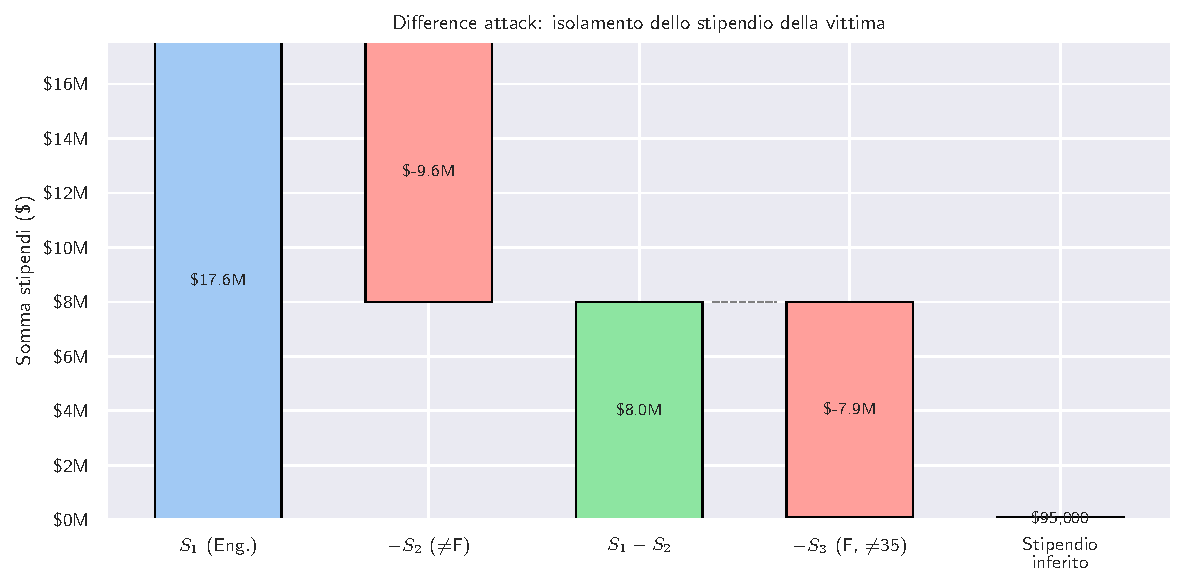
\includegraphics[width=0.65\linewidth]{plots/difference_attack_waterfall.pdf}
    \caption{Fasi del difference attack: le sottrazioni successive isolano il contributo della vittima}
    \label{fig:diff_waterfall}
\end{figure}

\subsection{Dataset sperimentale}

Per condurre l'esperimento, è stato generato un dataset sintetico che simula i dati dei dipendenti di un'azienda. L'obiettivo principale è dimostrare l'efficacia della privacy differenziale contro il differencing attack in condizioni controllate e verificabili. Questo richiede la garanzia che siano soddisfatte le condizioni necessarie al successo dell'attacco: la vittima deve essere univocamente identificabile tramite la combinazione di attributi noti all'attaccante; questa caratteristica, unita alla possibilità di calibrare con precisione i parametri di privacy, rende un dataset sintetico adatto agli scopi di questo esperimento.

Il dataset utilizzato è composto dalle informazioni di circa 500 dipendenti dove ogni record rappresenta un singolo dipendente, caratterizzato dai seguenti attributi:
\begin{itemize}
    \item \texttt{ID}
    \item \texttt{Department}
    \item \texttt{Age}
    \item \texttt{Gender}
    \item \texttt{YearsExperience}
    \item \texttt{Salary}, stipendio annuale
\end{itemize}

Per rendere la generazione del dataset realistica, sono state definite apposite distribuzioni di probabilità per l'assegnazione dei reparti e soglie plausibili per i valori di età, esperienza e stipendio, calibrandoli in base al reparto di appartenenza. Per le configurazioni esatte, consultare il codice allegato.

Si riportano di seguito le informazioni relative alla vittima che l'attaccante ha ottenuto tramite l'analisi di fonti di dati ausiliarie:
\begin{itemize}
    \item genere: femminile
    \item reparto lavorativo: engineering
    \item età: 35 anni
\end{itemize}
Queste sono informazioni facilmente ottenibili tramite piattaforme come Linkedin o altri social network; queste informazioni, combinate con la conoscenza della struttura del dataset, permettono all'attaccante di definire una serie di query da eseguire sul database per condurre un \textit{difference attack}.

In aggiunta a queste informazioni, si è deciso di impostare lo stipendio della vittima a \$95,000: questo è il valore che l'attaccante mira a de-anonimizzare.

\section{Configurazione dell'esperimento e risultati}

L'esperimento valuta l'efficacia della protezione DP al variare del parametro $\varepsilon$, mantenendo costante $\delta = 1e-5$ ($<< 1/n$); i valori di epsilon scelti per eseguire l'esperimento corrispondono a quattro livelli di privacy: alto ($\varepsilon = 0.5$), moderato ($\varepsilon = 5$), medio ($\varepsilon = 10$) e basso ($\varepsilon = 15$).

La scelta del valore di $\varepsilon$ rappresenta un problema aperto nella comunità della privacy differenziale \cite{epsilonchoice}. Non esistono linee guida universali e la scelta dipende fortemente dalla sensibilità dei dati, così come dal dominio: a seconda del tipo di dati trattati, quantità diverse di rumore possono essere più o meno accettabili. Questo concetto verrà discusso ulteriormente in seguito.

L'aggregazione differenzialmente privata è configurata tramite il formato DPYaml, specificando il meccanismo di rumore Laplace (\texttt{noise\_kind: laplace}), l'identificatore di privacy (\texttt{id\_field: ID}) e la suddivisione del budget (\texttt{aggregation\_share: 0.9}), che destina il 90\% del budget all'aggregazione e il restante 10\% alla selezione della partizione.

Per eseguire il difference attack attraverso GoDP, ciascuna delle tre query dell'attacco viene configurata con una specifica DPYaml con i filtri corrispondenti. Tramite la sezione \texttt{filters} di DPYaml si specificano condizioni di selezione applicate al dataset prima di effettuare l'aggregazione DP specificata, permettendo all'attaccante di eseguire le stesse query che effettuerebbe sul database non protetto.

Per ogni valore di $\varepsilon$, sono state generate tre configurazioni distinte, una per ciascuna query $S_1$, $S_2$, $S_3$, per un totale di 12 esecuzioni ($4$ valori di $\varepsilon \times 3$ query).

L'operazione di aggregazione utilizzata (\texttt{sum\_per\_key}) calcola la somma degli stipendi per reparto. I parametri di configurazione specificano che ogni dipendente appartiene a un solo reparto e contribuisce a una sola categoria (\texttt{max\_categories\_contributed: 1}) e una sola volta (\texttt{max\_contributions\_per\_category: 1}), con valori di stipendio compresi tra \$30,000 e \$200,000.

La sensitività globale dell'operazione di somma è determinata dall'intervallo dei possibili valori:
\begin{equation}
    \Delta f = \texttt{max\_value} - \texttt{min\_value} = 200{,}000 - 30{,}000 = 170{,}000
    \label{eq:exp_sensitivity}
\end{equation}

Il parametro di scala della distribuzione di Laplace, considerando che il 90\% del budget è allocato all'aggregazione, è:
\begin{equation}
    b = \frac{\Delta f}{\varepsilon_{\text{agg}}} = \frac{170{,}000}{0.9\varepsilon} = \frac{188{,}889}{\varepsilon}
    \label{eq:laplace_scale}
\end{equation}

In assenza di protezione DP, l'attacco di differenza ha successo con precisione del 100\%, l'attaccante riesce a dedurre esattamente lo stipendio della vittima, identificando un unico individuo che corrisponde alla combinazione di attributi nota. Questo risultato dimostra la vulnerabilità della combinazione delle aggregazioni non protette: utilizzando esclusivamente query aggregate, l'attaccante è in grado di determinare con certezza il valore sensibile di un individuo specifico.

\subsection{Attacco senza protezione DP}

In assenza di protezione DP il sistema restituisce i risultati esatti delle aggregazioni, le tre query dell'attaccante producono i seguenti risultati:
\begin{itemize}
    \item $S_1 = \$17,558,674$, somma degli stipendi di 157 dipendenti del reparto Engineering
    \item $S_2 = \$9,568,613$, somma degli stipendi di 87 dipendenti maschi del reparto Engineering
    \item $S_3 = \$7,895,061$, somma degli stipendi di 69 donne nel reparto Engineering con età diversa da 35
\end{itemize}

Applicando il calcolo \eqref{eq:inferred_salary}:
\begin{equation}
    \text{Stipendio}_{\text{vittima}} = (S_1 - S_2) - S_3 = (17{,}558{,}674 - 9{,}568{,}613) - 7{,}895{,}061 = \$95{,}000
\end{equation}

L'attaccante riesce a dedurre lo stipendio esatto della vittima, pari al valore reale \$95,000; questo mostra come il sistema, protetto solamente tramite la soppressione di query che restituiscono un numero di risultati inferiore a una soglia $k$, sia vulnerabile a questo tipo di attacco.

\subsection{Attacco con protezione DP}

Si ripete lo stesso attacco attraverso GoDP, che applica il meccanismo di Laplace alle aggregazioni. I risultati sono riassunti nella tabella seguente.

\begin{table}[H]
\centering
\caption{Risultati del difference attack con protezione DP al variare di $\varepsilon$.}
\label{tab:dp_results}
\begin{tabular}{l|c|c|c|c}
    \hline
    & $\varepsilon = 0.5$ & $\varepsilon = 5$ & $\varepsilon = 10$ & $\varepsilon = 15$ \\
    \hline
    $S_1$ DP & \$17{,}302{,}307 & \$17{,}549{,}307 & \$17{,}571{,}821 & \$17{,}571{,}068 \\
    $S_2$ DP & rimossa & \$9{,}625{,}483 & \$9{,}581{,}561 & \$9{,}556{,}128 \\
    $S_3$ DP & rimossa & \$7{,}879{,}474 & \$7{,}899{,}952 & \$7{,}899{,}090 \\
    \hline
    Stipendio inferito & -- & \$44{,}350 & \$90{,}308 & \$115{,}850 \\
    Errore assoluto & -- & \$50{,}650 & \$4{,}692 & \$20{,}850 \\
    Errore relativo & -- & 53.3\% & 4.9\% & 21.9\% \\
    \hline
    Protezione & massima & moderata & sufficiente & sufficiente \\
    \hline
\end{tabular}
\end{table}

\subsubsection{$\varepsilon = 0.5$: rimozione della partizione}

Per $\varepsilon = 0.5$ il meccanismo di partition selection rimuove completamente le partizioni delle query $S_2$ e $S_3$: i risultati di queste query non vengono restituiti dal sistema. In questo caso il budget $\varepsilon$ destinato alla partition selection ($0.1 \times 0.5 = 0.05$) è insufficiente a mantenere le partizioni che contengono un numero ridotto di record, impedendo del tutto il calcolo delle differenze necessarie all'attacco.

Questo risultato evidenzia come la selezione delle partizioni agisca come un ulteriore livello di protezione, infatti per valori molto bassi di $\varepsilon$ il meccanismo non si limita ad aggiungere rumore alle aggregazioni, ma impedisce la pubblicazione dei risultati di query che coinvolgono gruppi di dimensione ridotta. L'attaccante non è in grado di eseguire il differencing attack in quanto non dispone dei dati necessari al calcolo. Questo fenomeno è coerente con le garanzie teoriche della DP: una $\varepsilon$ molto stringente può portare a una perdita completa di utilità dei dati.

\subsubsection{$\varepsilon = 5$: protezione moderata}

Per $\varepsilon = 5$ tutte le query restituiscono risultati, ma il rumore composto attraverso le sottrazioni successive porta l'attaccante a inferire uno stipendio di \$44,350, risultato che esibisce un errore del 53.3\% rispetto allo stipendio reale della vittima. La composizione del rumore è un effetto fondamentale, dato che lo stipendio è calcolato come $(S_1 - S_2) - S_3$, il rumore delle tre query viene sommato.

\subsubsection{$\varepsilon = 10$ e $\varepsilon = 15$: protezione ridotta}

Per $\varepsilon = 10$ l'attaccante inferisce un valore di \$90,308 con un errore del 4.9\%; per $\varepsilon = 15$ il valore inferito è di circa \$115,850 con un errore del 21.9\%. In entrambi i casi il rumore aggiunto alle singole query è ridotto rispetto al caso precedente.

L'errore finale dipende dalla composizione algebrica delle quantità di rumore, questa caratteristica può portare sia a sovrastime che sottostime del valore reale.

Questi valori di $\varepsilon$ offrono una protezione limitata, lo stipendio inferito è sufficientemente vicino al valore reale da permettere all'attaccante di ottenere un'approssimazione ragionevole del dato sensibile.

\begin{figure}[H]
    \centering
    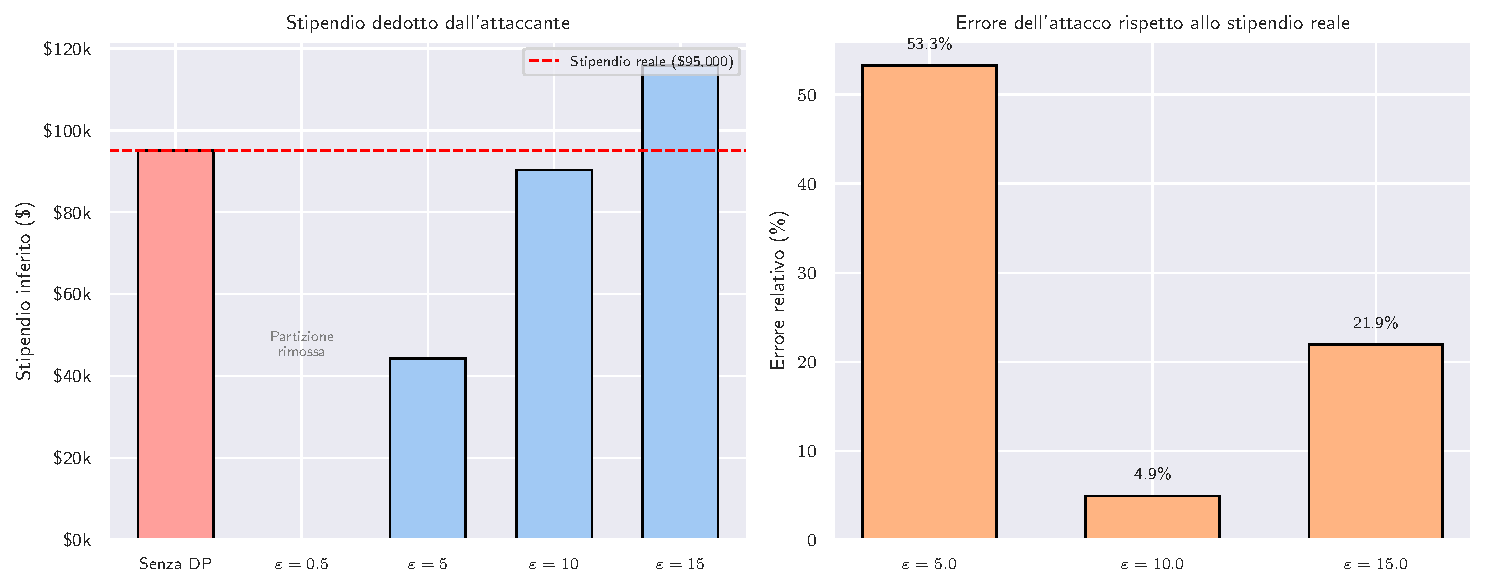
\includegraphics[width=0.8\linewidth]{plots/attack_comparison.pdf}
    \caption{Confronto tra i risultati dell'attacco con e senza protezione DP (sinistra) e errore relativo al variare di $\varepsilon$ (destra)}
    \label{fig:attack_comparison}
\end{figure}

\subsection{Analisi del rumore}

Il rumore aggiunto dal meccanismo di Laplace a ciascuna query è determinato dal parametro di scala $b = \Delta f / \varepsilon_{\text{agg}}$ (equazione \eqref{eq:laplace_scale}).

La tabella \ref{tab:abs_noise} riporta il rumore assoluto misurato su ciascuna query per i valori di $\varepsilon$ per i quali tutte le query restituiscono un risultato.

\begin{table}[H]
    \centering
    \begin{tabular}{l|c|c|c|c}
        \hline
        & $b$ (teorico) & $|\text{Rumore } S_1|$ & $|\text{Rumore } S_2|$ & $|\text{Rumore } S_3|$ \\
        \hline
        $\varepsilon = 5$  & \$37{,}778 & \$9{,}367 & \$56{,}870 & \$15{,}587 \\
        $\varepsilon = 10$ & \$18{,}889 & \$13{,}147 & \$12{,}948 & \$4{,}891 \\
        $\varepsilon = 15$ & \$12{,}593 & \$12{,}394 & \$12{,}485 & \$4{,}029 \\
        \hline
    \end{tabular}
    \caption{Rumore assoluto (\$) aggiunto alle singole query dal meccanismo di Laplace.}
    \label{tab:abs_noise}
\end{table}


Si osserva come con la diminuzione di $\varepsilon$ il parametro di scala $b$ cresca, portando a valori di rumore composto di ampiezza mediamente maggiore, anche se questo risultato non è costante in quanto si utilizzano valori campionati da una distribuzione di probabilità.

La figura \ref{fig:noise_vs_epsilon} mostra il rumore registrato per ciascuna query al variare di $\varepsilon$, insieme all'andamento teorico del parametro di scala.

\begin{figure}[H]
    \centering
    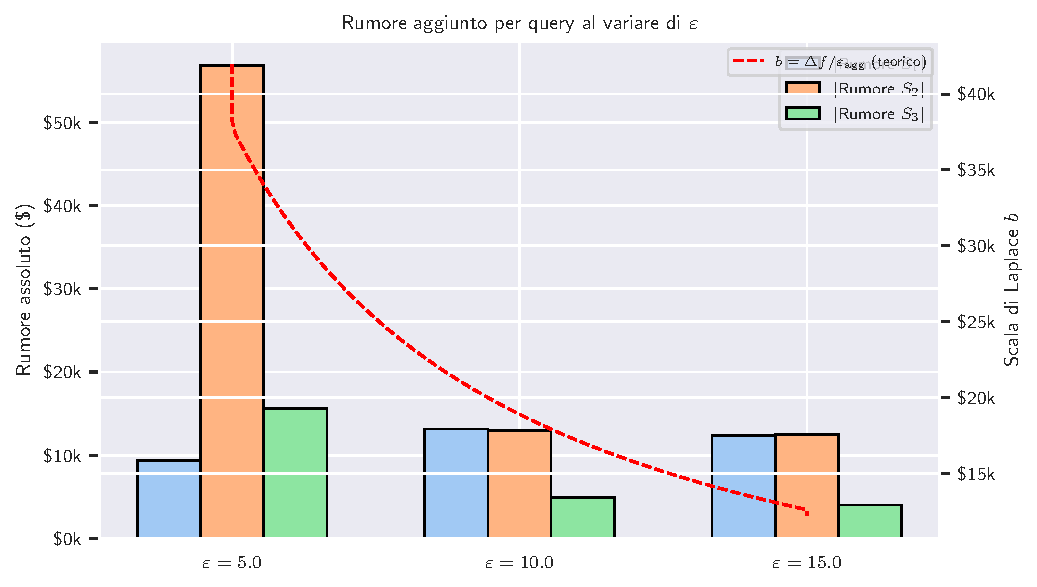
\includegraphics[width=0.8\linewidth]{plots/noise_vs_epsilon.pdf}
    \caption{Rumore assoluto per query al variare di $\varepsilon$ a confronto con il parametro di scala teorico $b = \Delta f / \varepsilon_{\text{agg}}$}
    \label{fig:noise_vs_epsilon}
\end{figure}

Un aspetto critico dell'attacco è la composizione del rumore attraverso le operazioni di sottrazione. Lo stipendio inferito è calcolato come $(S_1 - S_2) - S_3$, denotando con $\eta_i$ il rumore sulla query $S_i$, il rumore composto sul risultato finale è:
\begin{equation}
    \eta_{\text{tot}} = \eta_1 - \eta_2 - \eta_3
    \label{{eq:noise_comp}}
\end{equation}

Poiché le variabili $\eta_i$ sono indipendenti e distribuite secondo $\text{Lap}(0, b)$, la varianza del rumore composto è:
\begin{equation}
    \text{Var}(\eta_{\text{tot}}) = 3 \cdot \text{Var}(\eta_i) = 3 \cdot 2b^2 = 6b^2
    \label{eq:noise_variance}
\end{equation}

Questo significa che la deviazione standard del rumore composto è $\sigma_{\text{tot}} = b\sqrt{6} \approx 2.45b$, indicando come l'esecuzione di tre query amplifichi significativamente l'incertezza rispetto a una singola query.

\section{Discussione}

I risultati sperimentali illustrano il trade-off fondamentale tra privacy e utilità che caratterizza la privacy differenziale.

L'esperimento mostra un comportamento coerente con le proprietà teoriche della DP, al diminuire di $\varepsilon$, la protezione contro l'attacco di de-anonimizzazione aumenta. Per $\varepsilon = 0.5$ l'attacco è neutralizzato dalla rimozione delle partizioni, insieme all'utilità stessa dei dati. Per $\varepsilon = 5$ il rumore composto rende l'inferenza inaffidabile con errore del 53.3\%; per valori più elevati di $\varepsilon$ ($10$, $15$) la protezione è mantenuta in quanto l'attaccante non riesce a dedurre lo stipendio esatto ma i dati mantengono un certo livello di utilità.

\subsection{Selezione della partizione}

I risultati evidenziano il ruolo della partition selection come componente di protezione complementare al rumore; il budget allocato alla partition selection (10\% del totale) sottrae budget alla privacy, aumentando la quantità di rumore aggiunta alle aggregazioni, ed agisce come filtro che esclude dalla pubblicazione le aggregazioni su gruppi di dimensione ridotta. Nel caso con $\varepsilon = 0.5$ questo meccanismo costituisce il fattore principale del fallimento del differencing attack: le query $S_2$ e $S_3$, che filtrano per attributi specifici e producono gruppi molto ridotti, vengono rimosse dal meccanismo prima ancora che agisca il meccanismo di addizione del rumore.

\subsection{Limitazioni dell'esperimento}

L'esperimento presenta alcuni limiti che è opportuno evidenziare. In primo luogo, i risultati riportati corrispondono a una singola esecuzione del meccanismo DP, dato che il meccanismo DP si basa su un processo stocastico, esecuzioni diverse portano a risultati diversi e l'errore osservato può variare significativamente. Un'analisi statistica su molteplici esecuzioni permetterebbe di caratterizzare la distribuzione degli errori in modo più accurato; tuttavia è opportuno considerare che il budget di privacy utilizzato è da considerarsi "esaurito", in quanto ogni rilascio di dati dal sistema accumula il budget di privacy utilizzato associato a un determinato dataset.

Infine, il dataset è sintetico e progettato per garantire le condizioni di successo dell'attacco (unicità della vittima). In contesti reali, fattori come la dimensione del dataset, la distribuzione degli attributi e la complessità dello schema possono influenzare sia la fattibilità dell'attacco sia l'efficacia della protezione DP.